\section{実験}

口から鼻に抜ける香り(レトロネーザル)からの嗅覚情報の提示方法として,アガーを使用し
たゼリーを用いた.アガーを使用したゼリーを球体に固め,その中身を空洞にすることで空気を
入れるスペースが出来る.スペースに香りを閉じこめることで香りを閉じこめたゼリーを作成し
た.そのゼリーを口から食べることで口の中でゼリーが割れることにより,閉じこめられていた
香りが出て鼻から抜ける香りを与える物となっている.

\subsection{風味変容システムの概要}

嗅覚情報を風味として付与する仕組みとして,
香りの付いた液体を熱する事で出る蒸気を吸い,
その香りを楽しむVapeの香料の液体であるリキッドを
使用した.
気化させた香料を中に閉じこめる風味強化した新たなシステムを試作している.アルコー
ルのような気化しやすい液体を混ぜて中に入れゼリーの中で気化して充満させることでより香料
の濃度を上がることが出来ると考えた.


\subsection{ゼリーの大きさと作成}

中に香りを閉じこめるためには,ゼリーの中身を空洞にする必要がある.そのため,ゼリーを
作成するための材料といてアガーを使用した.今回アガーを利用した理由は,ゼラチンよりも透
明度が高く,常温でも溶けない性質を持っているからである.また,アガー自体には味がついてお
らずゼリー状に固めても無味無臭で作ることが出来る.もう一つの特徴として,溶ける温度が 90
℃以上と溶けにくく,固まる温度が30,40℃と常温でも固まりすぐに固めることが出来るため
扱いやすく丈夫である.固める際にで示した丸い氷を作成する用の製氷機を使用した.


ゼリーは直径3センチメートルの大きさの製氷機を使用し作成した.
安全に口内に入れやすく香料を入れる容量があるで示した直径3センチメー
トルの製氷機を使用した.


また,ゼリーを作成するにおいて予備実験から強度が弱く中に香りを入れる際に穴を開けるた
め潰れてしまう問題点が存在した.そのため,強度が強いものにするために氷水で5分間冷や
した後冷蔵庫で冷やすことでより図\ref{zeri}で示した強度の強いゼリーを作り出すことができた.ゼ
リー作成方法は以下のようになっている.


1.  アガー 5g を鍋に入れ,水 100ml を少しずつ混ぜながら加える.


2.  完全に解けたら火にかける.沸騰したら火を止める.


3. 2 の液体を立体の体積の半分よりやや少なめに入れる.


4.  フタをして,開かないように固定.


5.  容器を氷水の中で5分ほど回す. この時に一定方向だけでなく縦横斜めと全体にいきたわるように回す.


6.  冷蔵庫で冷やしておく. 冷やしておく事でゼリーがより固まり取り出しやすくなる.



  \begin{figure}[t]
    \centering
    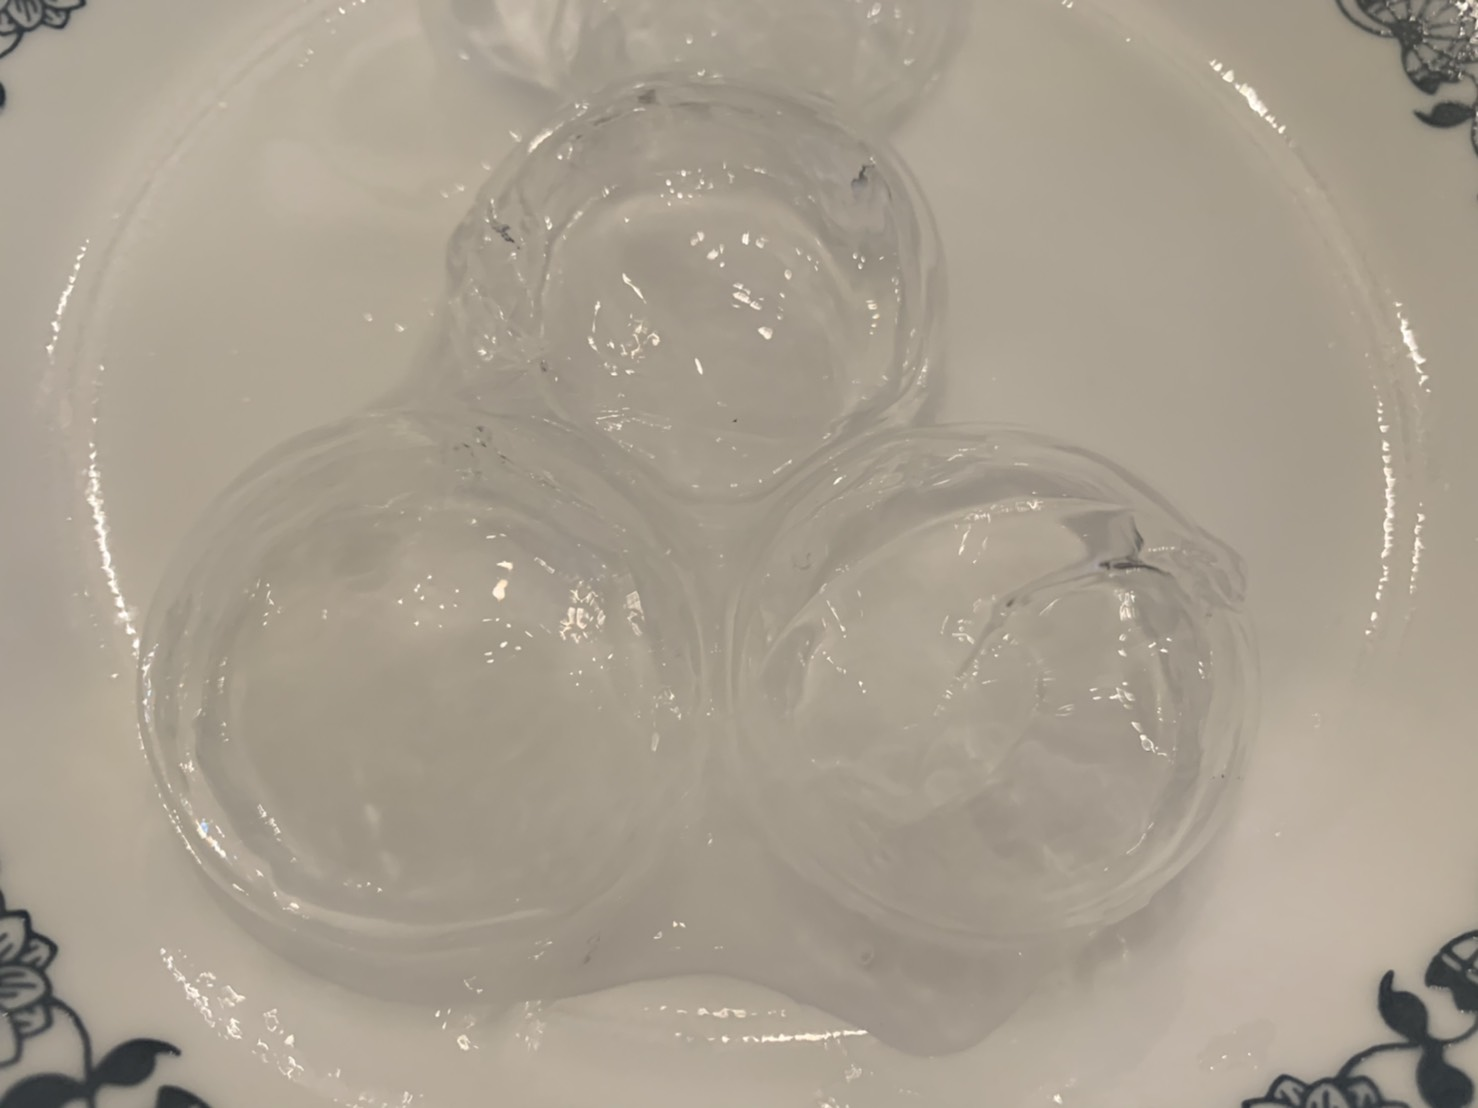
\includegraphics[width = 0.7\columnwidth]{zeri2.jpg}
    \caption{空洞のあるゼリー}
    \label{zeri}
  \end{figure}


\subsection{香りの注入方法}
  空洞があるゼリーに香りを閉じこめるために,大きな穴が開かないよう
に図\ref{tyusya}で示した細い針の注射器を使用した.元々空洞に空気がはいっているため注射器でゼ
リーの空洞の空気を抜くことにより中に香りをこめた空気が入るようにして,注射器で香りを空
洞の中に注入した.

\begin{figure}[t]
  \centering
  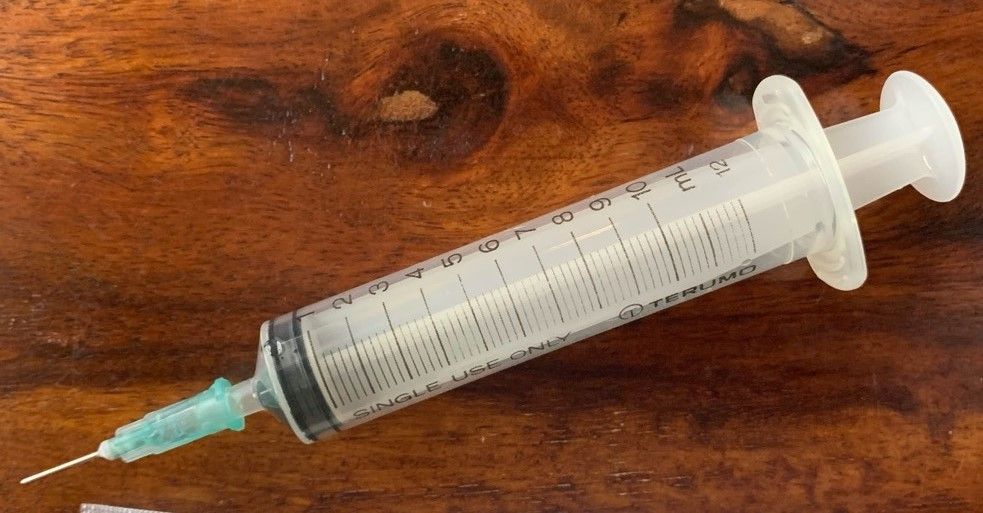
\includegraphics[width = 0.8\columnwidth]{tyusya1.jpg}
  \caption{香りを注入する注射器}
  \label{tyusya}
\end{figure}


\subsection{実験の方法}

本実験では香りを閉じこめた直径3センチメートルのゼリーを食べることで,風味を想起させ
ることが出来るかを検討する.香りを想起させるためにVapeの香りがわかりやすいリキッド二
つの香りを用意した.なお,口内で香りを充満させ風味を感じさせるために食べる際にゼリーを
口内で割るよう一口で口内に入れてもらう.この時に舌に当たる味ではなく鼻から向ける風味を
感じることができるかを判断してもらう.今回の実験では,作成した嗅覚提示ゼリーの有用性を
調査するとともに,中に入れる香りがどの程度の認知を得るか調査した.


今回実験するにあたって四種類のゼリーを用意した.香料を気化させた空気を注射器で吸い取
り,空洞のゼリーに入れたものを青りんごの Vape リキッドとバニラエッセンスの二
種類用意した.この青りんごの香りを含んだゼリーを1のゼリー,バニラの香りを含んだゼリー
を2のゼリーとする.


また,香料をゼリーの中に入れ,ゼリー内で気化させ中に香りを充満させる方法で青りんごの
Vapeリキッドとバニラエッセンスの二種類用意した. この青りんごの香りを含んだゼリーを3の
ゼリーバニラの香りを含んだゼリーを4のゼリーとする.
この四種類の香りの入ったゼリーを食してもらい風味の感じ方を調査した.